\documentclass[journal,12pt,twocolumn]{IEEEtran}

\usepackage{setspace}
\usepackage{gensymb}

\singlespacing


\usepackage[cmex10]{amsmath}

\usepackage{amsthm}

\usepackage{mathrsfs}
\usepackage{txfonts}
\usepackage{stfloats}
\usepackage{bm}
\usepackage{cite}
\usepackage{cases}
\usepackage{subfig}

\usepackage{longtable}
\usepackage{multirow}

\usepackage{enumitem}
\usepackage{mathtools}
\usepackage{steinmetz}
\usepackage{tikz}
\usepackage{circuitikz}
\usepackage{verbatim}
\usepackage{tfrupee}
\usepackage[breaklinks=true]{hyperref}
\usepackage{graphicx}
\usepackage{tkz-euclide}

\usetikzlibrary{calc,math}
\usepackage{listings}
    \usepackage{color}                                            %%
    \usepackage{array}                                            %%
    \usepackage{longtable}                                        %%
    \usepackage{calc}                                             %%
    \usepackage{multirow}                                         %%
    \usepackage{hhline}                                           %%
    \usepackage{ifthen}                                           %%
    \usepackage{lscape}     
\usepackage{multicol}
\usepackage{chngcntr}

\DeclareMathOperator*{\Res}{Res}

\renewcommand\thesection{\arabic{section}}
\renewcommand\thesubsection{\thesection.\arabic{subsection}}
\renewcommand\thesubsubsection{\thesubsection.\arabic{subsubsection}}

\renewcommand\thesectiondis{\arabic{section}}
\renewcommand\thesubsectiondis{\thesectiondis.\arabic{subsection}}
\renewcommand\thesubsubsectiondis{\thesubsectiondis.\arabic{subsubsection}}


\hyphenation{op-tical net-works semi-conduc-tor}
\def\inputGnumericTable{}                                 %%

\lstset{
%language=C,
frame=single, 
breaklines=true,
columns=fullflexible
}
\begin{document}


\newtheorem{theorem}{Theorem}[section]
\newtheorem{problem}{Problem}
\newtheorem{proposition}{Proposition}[section]
\newtheorem{lemma}{Lemma}[section]
\newtheorem{corollary}[theorem]{Corollary}
\newtheorem{example}{Example}[section]
\newtheorem{definition}[problem]{Definition}

\newcommand{\BEQA}{\begin{eqnarray}}
\newcommand{\EEQA}{\end{eqnarray}}
\newcommand{\define}{\stackrel{\triangle}{=}}
\bibliographystyle{IEEEtran}
\providecommand{\mbf}{\mathbf}
\providecommand{\pr}[1]{\ensuremath{\Pr\left(#1\right)}}
\providecommand{\qfunc}[1]{\ensuremath{Q\left(#1\right)}}
\providecommand{\sbrak}[1]{\ensuremath{{}\left[#1\right]}}
\providecommand{\lsbrak}[1]{\ensuremath{{}\left[#1\right.}}
\providecommand{\rsbrak}[1]{\ensuremath{{}\left.#1\right]}}
\providecommand{\brak}[1]{\ensuremath{\left(#1\right)}}
\providecommand{\lbrak}[1]{\ensuremath{\left(#1\right.}}
\providecommand{\rbrak}[1]{\ensuremath{\left.#1\right)}}
\providecommand{\cbrak}[1]{\ensuremath{\left\{#1\right\}}}
\providecommand{\lcbrak}[1]{\ensuremath{\left\{#1\right.}}
\providecommand{\rcbrak}[1]{\ensuremath{\left.#1\right\}}}
\theoremstyle{remark}
\newtheorem{rem}{Remark}
\newcommand{\sgn}{\mathop{\mathrm{sgn}}}
\providecommand{\abs}[1]{\left\vert#1\right\vert}
\providecommand{\res}[1]{\Res\displaylimits_{#1}} 
\providecommand{\norm}[1]{\left\lVert#1\right\rVert}
%\providecommand{\norm}[1]{\lVert#1\rVert}
\providecommand{\mtx}[1]{\mathbf{#1}}
\providecommand{\mean}[1]{E\left[ #1 \right]}
\providecommand{\fourier}{\overset{\mathcal{F}}{ \rightleftharpoons}}
%\providecommand{\hilbert}{\overset{\mathcal{H}}{ \rightleftharpoons}}
\providecommand{\system}{\overset{\mathcal{H}}{ \longleftrightarrow}}
	%\newcommand{\solution}[2]{\textbf{Solution:}{#1}}
\newcommand{\solution}{\noindent \textbf{Solution: }}
\newcommand{\cosec}{\,\text{cosec}\,}
\providecommand{\dec}[2]{\ensuremath{\overset{#1}{\underset{#2}{\gtrless}}}}
\newcommand{\myvec}[1]{\ensuremath{\begin{pmatrix}#1\end{pmatrix}}}
\newcommand{\mydet}[1]{\ensuremath{\begin{vmatrix}#1\end{vmatrix}}}
\numberwithin{equation}{subsection}
\makeatletter
\@addtoreset{figure}{problem}
\makeatother
\let\StandardTheFigure\thefigure
\let\vec\mathbf
\renewcommand{\thefigure}{\theproblem}
\def\putbox#1#2#3{\makebox[0in][l]{\makebox[#1][l]{}\raisebox{\baselineskip}[0in][0in]{\raisebox{#2}[0in][0in]{#3}}}}
     \def\rightbox#1{\makebox[0in][r]{#1}}
     \def\centbox#1{\makebox[0in]{#1}}
     \def\topbox#1{\raisebox{-\baselineskip}[0in][0in]{#1}}
     \def\midbox#1{\raisebox{-0.5\baselineskip}[0in][0in]{#1}}
\vspace{3cm}
\title{Assignment 2}
\author{K.A. Raja Babu}
\maketitle
\newpage
\bigskip
\renewcommand{\thefigure}{\theenumi}
\renewcommand{\thetable}{\theenumi}
Download all python codes from 
\begin{lstlisting}
https://github.com/ka-raja-babu/Matrix-Theory/tree/main/Assignment2/Python Codes
\end{lstlisting}
%
and latex-tikz codes from 
%
\begin{lstlisting}
https://github.com/ka-raja-babu/Matrix-Theory/tree/main/Assignment2/LaTex Codes
\end{lstlisting}
%
\section{Question No. 32}
Can you construct a quadrilateral $PQRS$ with $PQ$ = 3,$RS$ = 3,$PS$ = 7.5,$PR$ = 8 and $SQ$ = 4 ?
%
\section{Solution}
\begin{enumerate}
    \item Assume vertices of given quadrilateral:-
    
    Let the vertices of quadrilateral $PQRS$ be $\vec{P}$,$\vec{Q}$,$\vec{R}$ and $\vec{S}$ .
    
    \item List out given data in form of vectors:-
    
    According to given data:
    \begin{align}
    \norm{\vec{P}-\vec{Q}} = 3
    \\
    \norm{\vec{R}-\vec{S}} = 3
    \\
    \norm{\vec{P}-\vec{S}} = 7.5
    \\
    \norm{\vec{P}-\vec{R}} = 8
    \\
    \norm{\vec{S}-\vec{Q}} = 4
    \end{align}
    
    \item Find out two triangles of given quadrilateral having same base
    
    Quadrilateral $PQRS$ is made up of two triangles $\triangle PSQ$ and $\triangle PSR$ placed on base $PS$ .
    
    \item Verify that construction of both triangles,is possible or not by using the fact that "sum of any two sides of a triangle is greater than third side":-
    
    Now,in $\triangle PSR$ :-
    \begin{align}
    \norm{\vec{P}-\vec{S}} + \norm{\vec{R}-\vec{S}} = 7.5 + 3 =10.5 > \norm{\vec{P}-\vec{R}}
    \\
    \norm{\vec{P}-\vec{R}} + \norm{\vec{R}-\vec{S}} = 8 + 3 =11 > \norm{\vec{P}-\vec{S}}
    \\
    \norm{\vec{P}-\vec{S}} + \norm{\vec{P}-\vec{R}} = 7.5 + 8 =15.5 > \norm{\vec{R}-\vec{S}}
    \end{align}

    $\because$ Sum of any two sides is greater than third side in $\triangle PSR$ .
    \\
    $\therefore$ Construction of $\triangle PSR$ is possible.

    Now,in $\triangle PSQ$ :-
    \begin{align}
    \norm{\vec{P}-\vec{S}} + \norm{\vec{S}-\vec{Q}} = 7.5 + 4 =11.5 > \norm{\vec{P}-\vec{Q}}
    \\
    \norm{\vec{P}-\vec{S}} + \norm{\vec{P}-\vec{Q}} = 7.5 + 3 =10.5 > \norm{\vec{S}-\vec{Q}}
    \\
    \norm{\vec{P}-\vec{Q}} + \norm{\vec{S}-\vec{Q}} = 3 + 4 =7 < \norm{\vec{P}-\vec{S}}
    \end{align}

    $\because$ ( $PQ$ + $SQ$ ) $<$ $PS$ in $\triangle PSQ$ .
    \\
    $\therefore$ Construction of $\triangle PSQ$ is not possible.
    
    \item Conclude that construction of quadrilateral is possible if both triangles can be constructed otherwise not possible:-
    \\
    Without $\triangle PSQ$ , quadrilateral $PQRS$ cannot be constructed.Hence,construction of quadrilateral $PQRS$ is not possible with the given values.
    
    \item Perform construction of quadrilateral to know why it cannot be constructed:-
    \\
    In fig. \ref{fig:const_quadrilateral},two arcs with centre $P$ and $S$ and radius 3 cm and 4 cm respectively , will never intersect each other at any point.So,point $Q$ will never be formed and hence,quadrilateral $PQRS$ will never be constructed.
    
    \numberwithin{figure}{section}
    \begin{figure}[!ht]
    \centering
    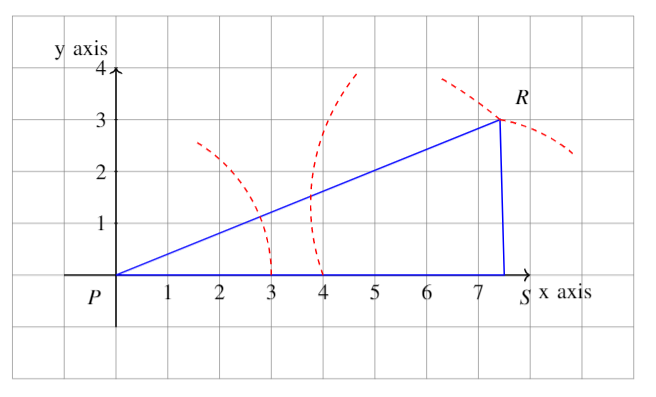
\includegraphics[width=\columnwidth]{Figure2}
    \caption{Construction of quadrilateral $PQRS$}
    \label{fig:const_quadrilateral}	
    \end{figure}
  
\end{enumerate}

\end{document}
